%!TeX program = xelatex
%!TeX builder = latexmk
\documentclass{mcmthesis}
\mcmsetup{tcn = 88277, problem = C}
\usepackage{blindtext}      % 提供 \blindtext 命令,演示用
\usepackage{subfigure}
\usepackage{caption}
\usepackage{csvsimple}
\usepackage{booktabs}
\usepackage{indentfirst}
\setlength{\parindent}{2em}

\title{The Title Energy}
\author{Team 88277}
\date{\today}

\begin{document}
% 摘要
\begin{abstract}
abstract content blablabla \\
next line
% 用 \\ 换行
% 关键字
\begin{keywords}
keyword1; keyword2
\end{keywords}

\end{abstract}

\maketitle                  % 生成前面的摘要页和标题页
\tableofcontents
% 介绍 Introduction
\section{Introduction}
Energy is a major issue in the world. Societies use energy for transportation, commercial, residential, industrial and domestic purpose.
%TODO: More backgrounds
In this paper, we propose a formula to describe the energy profile. We determine the metrics to represent the energy consumption and structure.
We select the related variables from the variable list.
Finally, we use the variable to describe the energy profile's formula, which shows the energy consumption and structure.
By analysing each state's status, we establish the energy profile for each state.
Then we build a multiple linear regression model with two variables, GDP (Gross domestic product) and population.
We use $MBE$ (Mean absolute error regression loss) and $R^2\ (coefficient\ of\ determination)\ regression\ score\ function$ to evaluate the model.
Then we forward a criteria to estimate the "best" profile for using cleaner, renewable energy.
We use four metrics and gathering the states's rank in each metric to find the best state.
Next, we find predict the energy profile in 2025 and 2050 for each state. After that we combine the prediction and criteria to form the targets for each state.
Accroding to the targets, we proposed five measures to rach the target.
% section
\section{Establishing Energy profile}
Our aim is to use the Energy profile to represent the total annual consumption of various energy
sources and their structure. According to introduction of the given data \cite{1},
we divide energy into five categories which are Coal, Natural Gas, Petroleum, Renewable Energy and Nuclear Electric Power.
This energy profile includes the annual consumption of five energy sources and describes their changes from 1960 to 2009.
In addition, we use the annual energy consumption of the five major energy sources
in different industries to reflect changes of energy structure.
\subsection{Data analysis and preparation}

\subsubsection{Energy classification}
Energy sources have been classified into five main kinds. Each kind energy is a set. Each set has one or more subcatorgories. The subcatorgories of each kind
have been listed in the memo page.%TODO: MEMO
\begin{itemize}
    \item Coal\\
    Includes coal ($CL$) and coal coke ($CC$). Recorded as $coal$ . Then $coal = \{CL, CC\}$
    \item Natural Gas\\
    Includes natural gas ($NN$). Recorded as $ng$ . Then $ng = \{NN\}$
    \item Petroleum\\
    Includes aviation gasoline ($AB$), crude oil ($CO$), fossile fuels ($ff$), jet fuel ($JF$) etc.
    Recorded as $petro$. Then $petro = \{AB, AR, AV, CO, DF, FF, FN, ... \}$. More variables are listed in the memo page.
    \item Renewable Energy\\
    Includes fuel ethanol ($EN$), geothermal energy ($GE$), solar energy ($GO$), wind ($WY$) and wood ($WD$) etc.
    Recorded as $re$ . Then $re = \{BM, EN, EM, ES, GE, GO, ... \}$
    \item Nuclear electric power\\
    Includes nuclear electric power ($NU$). Recorded as $nu$ . Then $nu = \{NU\}$
\end{itemize}
\subsubsection{Four kinds of industries}
\begin{itemize}
  \item Residential sector\\
  An energy-consuming sector that consists of living quarters for private households.\\
  We choose to use $RCB$ (residential energy consumption, data in British thermal units (Btu)) to measure its energy consumption.
  \item Commercial sector\\
  An energy-consuming sector that consists of service-providing facilities and equipment of: businesses; federal,
  state, and local governments; and other private and public organizations. \\
  We choose to use $CCB$ (commercial energy consumption, data in British thermal units (Btu)) to measure its energy consumption.
  \item Industrial sector\\
  An energy-consuming sector that consists of all facilities and equipment used for producing, processing, or assembling goods.\\
  We chose to use $ICB$ (Industrial energy consumption, data in British thermal units (Btu)) to measure its energy consumption.
  \item Transportation sector\\
  An energy-consuming sector that consists of all vehicles whose primary purpose is transporting people and/or
  goods from one physical location to another.\\
  We chose to use $TCB$ (Transportation energy consumption, data in British thermal units (Btu)) to measure its energy consumption.
\end{itemize}
\subsubsection{Formula calculation process}
\begin{itemize}
  \item Calculation of the total consumption of five kinds of energy sources
  Filter the given variables. What we need is the total annual consumption of each kind energy sources.
  For example, the total consumption of coal($coalTCB$) is $CLTCB + CCTCB$. \\
  The more general way to represent the total consumption of each kind energy sources is\\
  $$coalTCB = \sum_{i=0}^{n} var_iTCB  \ \ \ var_i \in coal, n = |coal| \\$$
  $$ngTCB = \sum_{i=0}^{n} var_iTCB  \ \ \ var_i \in ng, n = |ng| \\$$
  $$petroTCB = \sum_{i=0}^{n} var_iTCB  \ \ \ var_i \in petro, n = |petro| \\$$
  $$reTCB = \sum_{i=0}^{n} var_iTCB  \ \ \ var_i \in re, n = |re|$$
  $$nuTCB = \sum_{i=0}^{n} var_iTCB  \ \ \ var_i \in nu, n = |nu|$$
  \item Calculate the consumption of five kinds of energy sources in four sectors separately
  From the data, we choose the energy consumption of all energy sources in each sector and then add up according to the sector.
  For example, $coalRCB$ (consumption of coal in the residential sector) is: $CLRCB + CCRCB$ .
  As well, use symbols to represent this is
  $$coalACB = \sum_{i=0}^{n} var_iACB  \ \ \ var_i \in coal, n = |coal| \\$$
  $$coalCCB = \sum_{i=0}^{n} var_iCCB  \ \ \ var_i \in coal, n = |coal| \\$$
  $$coalICB = \sum_{i=0}^{n} var_iICB  \ \ \ var_i \in coal, n = |coal| \\$$
  $$coalRCB = \sum_{i=0}^{n} var_iRCB  \ \ \ var_i \in coal, n = |coal| \\$$
  And the rest three kinds of energy sources ($ng,\ petro,\ re\ and\ nu$) have similar formula.
\end{itemize}
\subsubsection{Formula for energy profile}
To get the final formula, we have one step to do. Use every kinds of annual consumption to divide it own fields of total annual consumption.
Such as, record the total energy annual consumption is $TETCB$, and the result of using $coalTCB$ to devide $TETCB$ is noted as $coalVT$.
$$coalVT = \frac{coalTCB}{TETCB}$$
And use $coalVA$ to record $coalACB$ to devide $TEACB$.
$$coalVA = \frac{coalACB}{TEACB}$$
More variables have been listed in the memo page.\\
The final representation of the formula is
$$
  EP =
  \begin{pmatrix}
  coalVT & coalVA & coalVC & coalVI & coalVR  \\
  ngVT & ngVA & ngVC & ngVI & ngVR \\
  petroVT & petroVA & petroVC & petroVI & petroVR \\
  reVT & reVA & reVC & reVI & reVR \\
  nuVT & 0 & 0 & 0 & 0\\
  \end{pmatrix}
$$

* Note that Nuclear Electric Power doesn't have variables to represent the annual consumption in different sectors.
But is still an important energy sources, so we keep it.

\subsection{California' energy profile}
California is the nation's third-largest state,and also California is the most populated state in the nation. Its total energy demand is second only to Texas.
California's extensive efforts to increase energy efficiency, along with the implementation of alternative technologies,
has restrained growth in energy demand. California is also rich in energy resources.
The state has an abundant supply of crude oil and is a top producer of conventional hydroelectric power.
California also leads the nation in electricity generation from solar, geothermal, and biomass resources.
\subsubsection{Petroleum}
  For California, oil is its primary source of energy, with oil accounting for more than $60\%$ of total energy consumption in the past 50 years.
  However, it can be seen that the share of oil in total consumption after constant technological innovation showing a weak downward trend.
  In the commercial and residential sectors, the proportion of oil used has risen to some extent, reaching around $40\%$ and $50\%$ in 2009.
  It shows that California is very dependent on oil. Although the overall trend is declining, it can not leave the oil in the short term.
\subsubsection{Natural gas}
  California accounts for less than $1\%$ of total U.S. natural gas reserves and production.
  After the 1970s, California's natural gas production experienced a gradual and complete decline over the past 30 years.
  From $30\%$ in the 1960s and now up and down at $20\%$.
  The demand for natural gas in California is not so strong, and from the data analysis, it has been relatively stable at about $20\%$ in recent years.
  The use of natural gas in the dwelling sector has dropped continuously from $80\%$ to $45\%$ in 50 years.
  The same is true of the commercial sector, which started to decline continuously after rising to $70\%$ in the 1970s and reached $25\%$ in 2009.
  Contrary to the previous one, the industrial sector seems to consider natural gas as a substitute for petroleum.
  After a decline in the 1970s, it rose from fluctuations in the mid-1980s to a $47\%$ share and is still on the rise.
\subsubsection{Renewable energy}
  California is among the top states in the nation in electricity generation from renewable resources and leads the nation in generation from solar, geothermal, and biomass energy.
  With the development of science and technology, the ratio of renewable energy sources shows a steady and steady rise in total energy consumption.
  This is evident in the residential and commercial sectors and has been rising for 50 years.
\subsubsection{Coal}
  California does not have any coal reserves or production and has phased out almost all use of coal for electricity generation.
  As you can see from the table, California's demand for coal is extremely low, even lower than the demand for renewable energy in 2000-2009.
  No matter in the commercial, transportation, residential or industrial sectors, there is an extremely low proportion of those coming out to zero and there is no continuing upward trend.
  \begin{figure}[htbp]
  \centering
  \begin{minipage}[t]{0.48\textwidth}
  \centering
  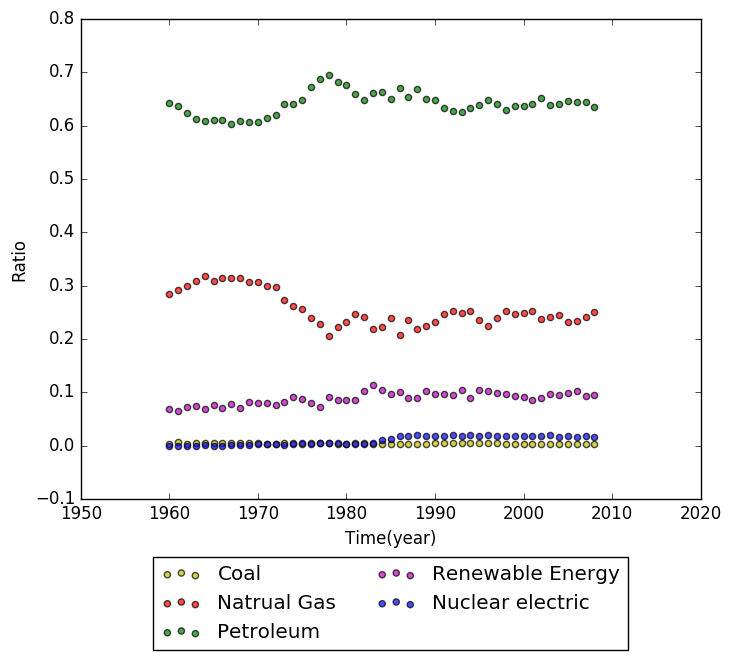
\includegraphics[width=6cm]{energyprofile_ca.png}
  \captionsetup{font={small}}
  \caption{Energy consumption, California}
  \end{minipage}
  \begin{minipage}[t]{0.48\textwidth}
  \centering
  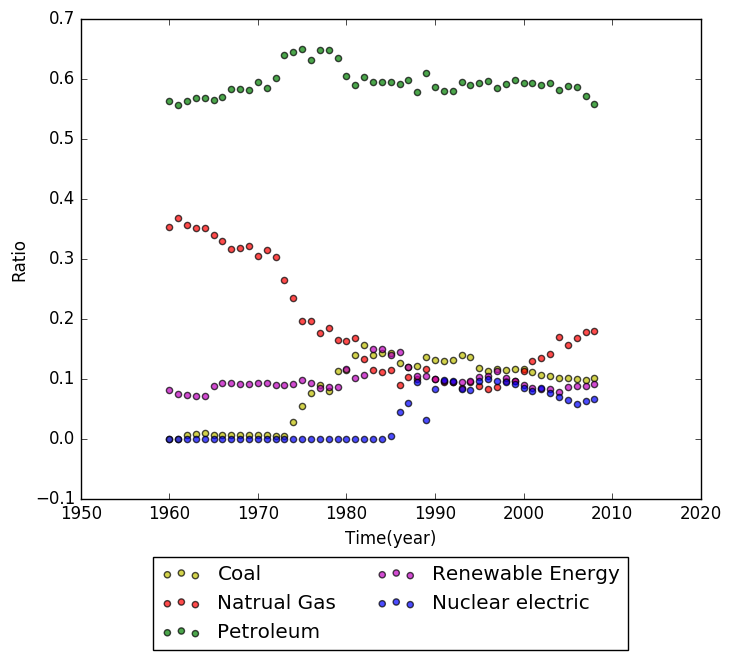
\includegraphics[width=6cm]{energyprofile_az.png}
  \captionsetup{font={small}}
  \caption{Energy consumption, Arizona}
  \end{minipage}
  \end{figure}
\subsection{Arizona' energy profile}
Arizona has few fossil fuel resources, but it does have abundant solar and geothermal energy potential. 
Elevations in Arizona vary from peaks more than 12,000 feet high in the north to nearly sea level in the lower deserts to the southwest.
And abundant sunshine gives the entire state some of the nation’s greatest solar power potential. 
The main energy source in Arizona is oil.
\subsubsection{Petroleum}
  Arizona does not have any refinery. Gasoline and other petroleum products are supplied by pipelines in Southern California and Texas.
  Since 2005, the share of renewable energy and natural gas has slightly declined. The use of oil in the industrial sector
  as a whole is on the rise, rising from $27\%$ to $65\%$ and is still on the rise. In the residential and commercial sectors, the share of
  oil also increased, with the residential sector rising from $16\%$ to $50\%$ and stabilizing, with $30\%$ of the commercial sector turning $52\%$.
  On the whole, Arizona is getting more and more dependent on oil.
\subsubsection{Natural gas}
  Arizona has no significant gas reserves. The share of natural gas from the 1960s to the 1990s has been declining until it showed an upward
  trend in the late 1990s. In all four sectors, natural gas consumption, in general, has been declining. In the commercial sector, the
  share of natural gas dropped rapidly from $64\%$ to below $10\%$.
  And fluctuated around $15\%$ in the 1990s and early twenty-first centuries. In the residential sector, the share of natural gas has been declining,
  from $70\%$ to $15\%$, and the post-term decline has been softer than the previous decline. In the transport sector from
  $22\%$ dropped to about $5\%$, and in 2009 by the rising trend.
\subsubsection{Renewable Energy}
  Arizona's renewable energy standards require that investors in the power utilities and retail power providers receive more and more electricity
  from renewable sources. Renewable energy has been one of Arizona's major energy sources and its share has been close to $10\%$ between the 1960s
  and the 1980s, with a sharp increase of nearly $15\%$ between 1980 and 1985. Since 2001, the share of renewable energy has risen
  slowly and has continued to rise. The share of renewable energy in the industry has been rising for 30 consecutive years, up to $20\%$ and
  a slight decrease since the 1990s. However, the proportion of renewable energy in the industries has been on a rising trend since the 21st century.
\subsubsection{Coal}
  Renewable energy Arizona has two coalfields - Black Mesa, the Navajo River and the Northeast Hippo Reservation, Pinedale, south-central Arizona.
  These areas maintain around $1\%$ of the country's coal reserves in producing mines. The only coal mine operating in the state is located in the Black
  Mesa field, one of the 30 largest coal mines in the country. Arizona started to use coal from the 1970s and quickly became a significant $12\%$ energy
  source in the 1980s. It began to slowly decline to $8\%$ (2009) in the early 1990's and remained stable. Industrial coal,
  which grew rapidly from the mid-1970s to the late 1980s, reached $20\%$ at one point and quickly dropped to $8\%$ in the early 1990s and remained stable.
\subsection{New Mexico's energy profile}
New Mexico is with much land but few people. Although it is the fifth-largest state by area, it is the sixth-least densely populated.
New Mexico is the nation's 7th largest net energy supply state, rich in fossil fuels, minerals and renewable energy resources.
The oil and gas industry, contributes significantly to the state's gross domestic product (GDP),
and workers in the sector earn among the highest average weekly pay in the state.
New Mexico's energy consumption per dollar of GDP and energy consumption per capita are both above the national average.
\subsubsection{Petroleum}
  New Mexico's crude oil reserves have surpassed $4\%$ of the U.S. The Permian Basin in western Texas and southeastern New Mexico are among
  the most productive oil producing areas in the country. The proportion of oil in total energy consumption is as high as more than half.
  From 1960, the proportion of petroleum energy consumption in New Mexico increased year by year, accounting for nearly $60\%$ by the 21st century.
  The industrial sector is far ahead, with only a small amount of oil being used in the residential and commercial sectors.
\subsubsection{Natural gas}
  New Mexico, accounting for about $5\%$ of the total natural gas reserves in the United States, is one of the top ten natural gas
  producers in the United States, accounting for about $4\%$ of the country's total natural gas production. Because of the high reserves of
  natural gas, natural gas accounted for as much as $45\%$ of the energy it consumed in the 1970s, comparable to oil.
  However, with the development of oil, coal and renewable energy, the proportion of natural gas in energy consumption has been declining year by year,
  reaching a minimum of $20\%$ in the mid-1980s. From 1990 to 2009, the proportion of natural gas consumption has fluctuated between $20\%$ and $25\%$
   and gradually stabilized.
\subsubsection{Renewable energy}
  New Mexico has a large number of renewable resources, especially wind and solar energy, as well as hydropower, biomass and geothermal energy.
  And it has developed rapidly in solar technology with the support of national policies. It can be seen that the proportion of energy
  consumption of renewable energy is gradually increasing, approaching $10\%$ by 2009 and there is a trend of continued growth.
  The proportion of energy consumption in the industrial, commercial and residential sectors has increased substantially.
  In particular, the energy consumption of renewable resources in commercial and residential sectors has exceeded $20\%$ by 2009.
\subsubsection{Coal}
  New Mexico contains nearly $3\%$ of the country's estimated recoverable coal reserves. New Mexico has mined coal since the 1850s.
  Therefore, from 1965 to 1985, the proportion of coal's energy consumption gradually increased, reaching a maximum of about $18\%$ in 1985.
  However, with the increase of renewable resources and oil, the proportion of coal's energy consumption has steadily declined.
  Through the analysis of energy consumption in the industrial, transportation, commercial and residential sectors,
  it can be seen that coal accounts for the smallest proportion of energy consumption in all sectors and shows a very small proportion of nearly zero.
  \begin{figure}[htbp]
  \centering
  \begin{minipage}[t]{0.48\textwidth}
  \centering
  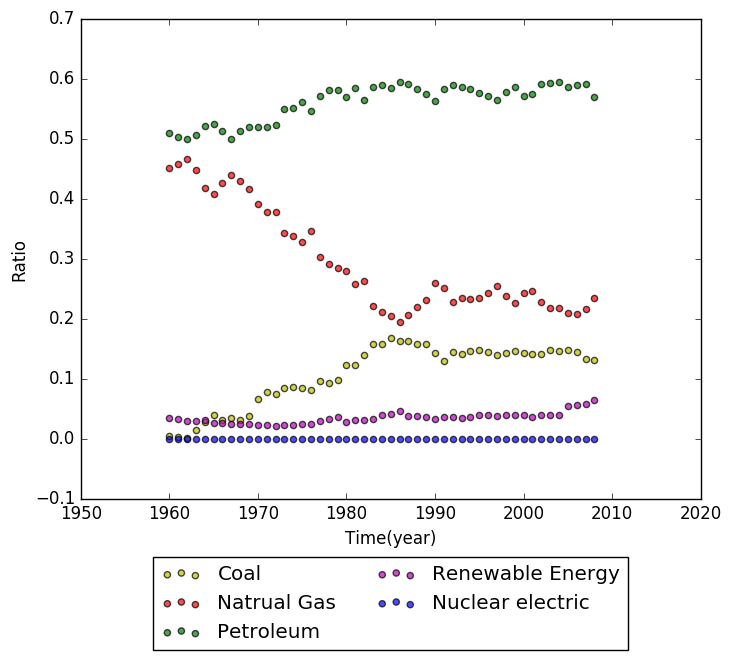
\includegraphics[width=6cm]{energyprofile_nm.png}
  \captionsetup{font={small}}
  \caption{Energy consumption, New Mexico}
  \end{minipage}
  \begin{minipage}[t]{0.48\textwidth}
  \centering
  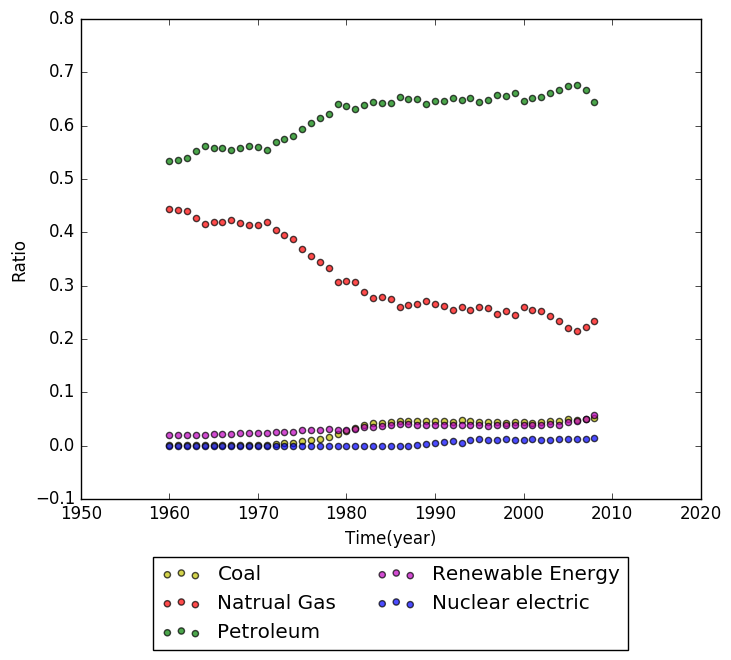
\includegraphics[width=6cm]{energyprofile_tx.png}
  \captionsetup{font={small}}
  \caption{Energy consumption, Texas}
  \end{minipage}
  \end{figure}
\subsection{Texas's energy profile}
Texas, located in the south-central part of the United States, is the second largest in size in the United States.
The Texas Almanac classifies the state into four regions: Gulf Coastal Plains, Interior Lowlands, Great Plains, and Basin and Range Province.
he Texas climate varies significantly from east to west. Moist air from the Gulf of Mexico sweeps westward across the state, losing moisture as it goes.
 As a result, the climate ranges from humid and subtropical along the coast, where much of the state's population resides, to semi-arid on the high plains, and arid in the mountainous west.
\subsubsection{Petroleum}
  Texas is a leader in crude oil reserves and production. More than a third of the U.S. crude oil has been proved reserves.
  From the discovery of the Spindletop field in 1901 to the subsequent discovery of various oil fields, the proportion of oil in Texas
  in energy consumption gradually increased to $63\%$ in 2009. The proportion of oil consumption is related to that of natural gas.
  The proportion of energy consumption in natural gas is correspondingly increased in the years in which the proportion of petroleum consumption
  is declining, and vice versa. In the industrial, commercial, transport and residential sectors, the proportion of oil in energy consumption is on the rise.
\subsubsection{Natural gas}
  Texas holds one-fourth of the nation's proved natural gas reserves and almost one-third of the 100 largest natural gas fields are located,
  n whole or in part, in the state. Texas also leads the nation in natural gas production, accounting for one-fourth of U.S. However,
  with the increase of oil, coal, renewable resources and nuclear resources, the energy consumption of natural gas has been on the
  whole declining from about $45\%$ in 1960 to about $25\%$ in 2009. In the industrial, commercial and residential sectors,
  by the mid-1970s, the share of natural gas in energy consumption was higher than that in oil, turning around in 1973,
  with the proportion of natural gas being exceeded by oil, and the gap between the two was growing.
\subsubsection{Renewable energy}
  Wind accounts for nearly all of the electricity generated from renewable resources in Texas. The size of the state and
  the high levels of direct solar radiation in West Texas give the state some of the largest solar power potential in the nation.
  The agricultural and forestry sectors can provide Texas with abundant biomass and biofuel resources.
  Despite the large number of non-powered dams in Texas, the potential for further hydroelectric development is limited by lack of precipitation.
  Besides, Texas has a unique untapped geothermal resource: its large network of crude oil and natural gas wells. 
  Renewable resources in Texas, the proportion of energy consumption increased year by year.
  In particular, the proportion of energy in the commercial and residential sectors has been as high as $25\%$ to $30\%$.
\subsubsection{Coal}
  Texas found large lignite coal mines in the narrow belt of Texas Gulf Coast, as well as bituminous coal deposits in north-central
  and southwestern Texas. Overall, the state estimates recoverable reserves of more than 9 billion tons.
  Texas is the seventh largest coal producer and the nation's largest lignite producer. Texas is the largest coal-consuming nation
  whose emissions of carbon dioxide and sulfur dioxide are mainly from electricity generation and the highest in the country.
  The proportion of coal's energy consumption is on the rise, reaching about $5\%$ by 2009. However, the proportion of coal in
  various sectors is the lowest among all other resources.
% TODO: Polish energy profile and cut some unimportant part

\section{Developing the Model}
\subsection{Assumption}
% 引用文献说明
According to Energy and Population \cite{2},
we found that Energy consumption ralated to GDP (Gross domestic product) and population.
$$Population + GDP per capita + Energy\ per\ unit\ of\ GDP = Energy$$
Hence we use these three variables to estimate energy consumption.
\subsection{Calculate the Model}
A linear regression model that contains more than one predictor variable is called a multiple linear regression model\cite{3}.
Although we use linear regression, we could also have quadratic variables by using a variable $x^2$  as one variable of multiple variables.
At first we use population and GDP as two variables to buid the model. The function can be writen as
$$EP = \alpha_0 + \alpha_1 * Population + \label_2 * GDP $$
In data preprocessing, We uniform the data by using $Standard\ score$ \cite{4}
to scale the data into $(0,1)$ .
We choose testing data and training data randomly from the data set as testing data being $20\%$. In the model evaluation, we use two metrics to estimate the result.
One is $MBE$ (Mean absolute error regression loss), the reason we choose $MBE$ over $MSE$ (Mean squared error regression loss) is that the data is small than 1.
If we use $MSE$, the difference of the error is hard to distinguish. Using this metric, the small the result is the better the prediction is.
Another metric is $R^2\ (coefficient\ of\ determination)\ regression\ score\ function$.
Best possible score is 1.0 and it can be negative (because the model can be arbitrarily worse).
After we read the paper mentioned the third variable $Energy per uint of GDP$, we build the second model.
$$EP = \alpha_0 + \alpha_1 * Population + \label_2 * GDP + \label_3 * Energy\ per\ uinit\ of\ GDP $$
% 用回归分析,解释为什么用;以及说明建模过程中的一些细节问题;
\subsection{The Model Results}
We compared the error of the two models. By compare the $R^2\ score$, we calculated the four states separately,
find that more than a half of the result of second model is better than the first model. %(TODO:insert table)

\begin{table}[!htbp]
\centering
\caption{Comparison of the two models}\label{tab:aStrangeTable}
\begin{tabular}{cc}
\toprule
State& The ratio of model2 is better than model1\\
\midrule
California& 0.7619047619047619 \\
Arizona& 0.8095238095238095 \\
New Mexico& 0.5238095238095238 \\
Texas& 0.6666666666666666 \\
\bottomrule
\end{tabular}
\end{table}

% figure
\begin{figure} [h]
\small
\centering
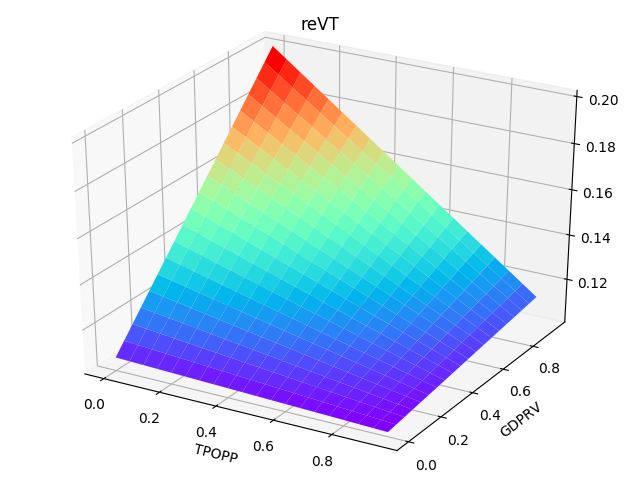
\includegraphics[width=12cm]{CA_reVT.png}
\caption{Renewable Energy Consumption's ralationship with GDP and Population} \label{fig:aa}
\end{figure}
%
% \begin{table}[!htbp]
% \centering
% \caption{a}\label{tab:aStrangeTable}
% \begin{tabular}{ccc}
% \toprule
% Variables& MBE& R^2\\
% \midrule
% Ch'en Meng& 001& Male\\
% Sarah Brightman& 002& Female\\
% \bottomrule
% \end{tabular}
% \end{table}
% \begin{table}[h!]
%   \centering
%   \caption{Model error for California}
%   \label{tab:table1}
%   \begin{tabular}{ccc}
%     \toprule
%     Variables & MBE & R^2\\
%     \midrule
%     coalVT	& 0.0008044891	& 0.0417302872 \\
%     coalVA	& 2.14623183534656E-06	& 0.4681465981\\
%     coalVC	& 0.000517853	& 0.3722870458 \\
%     coalVI	& 0.0040203466 & 0.25896736 \\
%     coalVR	& 9.6843507961811E-05	& -0.0425480067 \\
%     ngVT	& 0.0077195916	& 0.119103722 \\
%     ngVA	& 0.0008373601	& 0.6288560266 \\
%     ngVC	& 0.015049411	& 0.7549557304 \\
%     ngVI	& 0.0270951153	& 0.6848572025 \\
%     ngVR	& 0.0095303215	& 0.9545667853 \\
%     petroVT	& 0.0086889409	& 0.5007391906 \\
%     petroVA	& 0.0021181725	& 0.8153156324 \\
%     petroVC	& 0.0111721378	& 0.3467558584 \\
%     petroVI	& 0.031965453	& 0.5302410519 \\
%     petroVR	& 0.0064876244	& 0.9383029899 \\
%     reVT	& 0.0067068334	& 0.1888766313 \\
%     reVA	& 0.0013557953	& 0.8915757985 \\
%     reVC	& 0.0068823815	& 0.9201289253 \\
%     reVI	& 0.0072269526	& 0.7168082396 \\
%     reVR	& 0.0102720658	& 0.8322201492 \\
%     nuVT	& 0.0024848158	& 0.8121893345
%     \bottomrule
%   \end{tabular}
% \end{table}
%
% \begin{filecontents*}{model2.0_error_ca.csv}
% name,givenname,matriculation,gender,grade
% Maier,Hans,12345,m,1.0
% Huber,Anna,23456,f,2.3
% Weisbaeck,Werner,34567,m,5.0
% \end{filecontents*}
%
%     \begin{tabular}{l|c}%
%     \bfseries Person & \bfseries Matr.~No.% specify table head
%     \csvreader[head to column names]{model2.0_error_ca.csv}{}% use head of csv as column names
%     % {\\\hline\givenname\ \name & \matriculation}% specify your coloumns here
%     \end{tabular}

\section{Analysis based on the Model}
% Analyze and interpret the results of your model to address the four states’
% usage of cleaner, renewable energy sources in a way that is easily understood by the governors
% and helps them to understand the similarities and difference between the four states. Include in
% your discussion possible influential factors of the similarities and differences (e.g. geography,
% industry, population, and climate)
% 画出预测的图 分析和第一块有重复
\subsection{California}
California has deserts in the southeast, has a very abundant solar energy resources,
the same as California or the nation's third largest traditional hydroelectric state and the fifth largest wind power generation,
renewable energy power generation accounted for about $35\%$ of total power generation, the same natural gas power generation.
It is also increasingly becoming the main source of power generation in California.
It can be seen that the two sectors with the fastest growth and the largest proportion of use are the commercial sector and the residential sector.
This is closely linked with the government's active promotion of home use of solar energy and the construction of solar power plants and hydroelectric power stations in the desert.
In the same way, the share of renewable energy is hard to grow or slow to grow in the industrial and transport sectors, which requires technological innovations to promote the use of renewable energy.
California has the third largest oil field in the United States, and importing crude oil is not difficult, there is no tension in oil.
California is heavily dependent on oil resources, and particularly in the transportation and industrial sectors, the lack of oil supplies can have a significant impact on the state of California's economy,
but oil is a nonrenewable resource and all of California has taken steps to improve energy efficiency Approach to conserve the use of oil resources and reduce oil use as much as possible in the context of a unit of GDP,
not only saving resources but also increasing the share of renewable resources in total resources use. California accounts for less than $1\%$ of U.S. natural gas reserves and production.
With crude oil, California's natural gas production has been declining steadily over the past two decades.
Natural gas in California is mainly used for power generation and home heating, with per capita use of natural gas below the national average.
According to the chart, natural gas is less likely to fluctuate swiftly due to economic and demographic changes.
Therefore, the demand is relatively stable, requiring transportation and natural gas reserves. With no coal reserves or production in California.
California has phased out almost all coal used to generate electricity. California's dependence on coal is very low.
\subsection{Arizona}
The model mainly describes the impact of GDP and population on energy use. As can be seen, in Arizona, natural gas, renewable energy, coal and nuclear energy can replace each other, and in the past 50 years there is no good alternative to oil. The department that uses the most energy is the transport sector. Since automobiles do not have a good way of using clean energy, the proportion of oil in the transport sector can not be reduced while maintaining population and economy. The share of renewable energy in the commercial and residential sectors has risen rapidly. This is because Arizona has abundant solar energy resources. In this non-industrial sector, technological innovations for clean energy use are quicker and more rapidly applied. With the government's implementation, resources such as solar and wind energy can be efficiently used by residents use. Arizona has coal resources, so you can see that by the nineties, the share of coal resources was high, but due to the gradual depletion of coal resources and the Kyoto Protocol and other environmental protection documents, the government started to raise the level of clean energy Use and protect the environment, coal is the first to be abandoned energy use, indicating that the use of coal is not so irreplaceable. Arizona does not have a gas reserve and the overall per capita consumption of natural gas in Arizona is less than two-thirds of the states. It can be seen that the use of natural gas from the higher trend, there is this potential. The power industry is the most gas-consuming industry, so natural gas reserves and transportation are essential. The substitution of coal for thermal power generation by natural gas and the replacement of other energy sources by electricity can indirectly increase the proportion of clean energy in energy use.
\subsection{New Mexico}
In New Mexico, through the analysis of the model and the search for relevant information, it can be seen that the oil and natural gas industry have a significant contribution to the country's gross domestic product (GDP).
New Mexico's energy consumption per dollar of GDP and energy consumption per capita are both above the national average.
The higher reserves of crude oil and natural gas in New Mexico make it high in energy consumption for crude oil and natural gas.
Crude oil and natural gas have a high share of energy consumption in industry, commerce and transport.
Especially at the end of the twentieth century, as a result of the rapid growth of the transport industry, the share of oil energy consumption has risen sharply.
New Mexico contains nearly $3\%$ of the country's estimated recoverable coal reserves.
New Mexico has mined coal since the 1850s. However, with the development of other resources, the proportion of coal's energy consumption has been declining.
In terms of renewable resources, New Mexico has a large number of renewable resources, especially wind and solar energy, as well as hydropower, biomass and geothermal energy.
New Mexico has the sixth-largest geothermal resource in the country. New Mexico's climate is characterized by abundant sunshine, so the solar energy industry can be vigorously developed.
It can be seen that the proportion of energy consumption of renewable energy is gradually increasing, and the proportion of energy consumption in the industrial, commercial and residential sectors has increased substantially.
In particular, the energy consumption of renewable resources in the commercial and residential sectors has surged to 2009 Years are more than $20\%$.
The proportion of energy consumption in the future of renewable resources in New Mexico will increase in proportion to the trend of energy consumption.
And there are already relevant policies and industries, such as solar power, where the number of utility-scale solar PV installations in New Mexico is increasing and the number of distributed (customer-located, small-scale) solar power plants Use is also increasing.
National regulatory policies also strongly support the use of distributed solar technologies.
\subsection{Texas}
Through the analysis of the model and related data, we can see that Texas is the second largest population and the second largest economy after California.
The state leads the nation in total energy consumption, accounting for more than one-eighth of the U.S. total.
On a per capita basis, Texas is sixth in the nation in energy consumption.
Texas has many energy-intensive industries, including refining and chemical production, and accounts for the largest share of the industrial sector for the country's energy use.
The transport sector is the second most important part of energy consumption, partly because of the large number of cars registered because of the long distances across the country.
As a result, oil and gas resources account for the largest share of energy consumption in Texas. In addition, the share of renewable energy in Texas is increasing year on year.
In particular, the share of energy in the commercial and residential sectors has increased to as much as $25\%$.
In Texas, wind power accounts for almost all of the electricity from renewable sources. There are other renewable energy sources in Texas.
The size of West Texas and the high level of direct solar radiation provide the nation with the nation's largest solar potential.
The agriculture and forestry sector can provide Texas with abundant biomass and biofuel resources.
Texas has a unique undeveloped geothermal resource: its large crude oil and gas well network.
Existing wells are connected to deeper geothermal resources and many water temperatures can reach as high as 200 degrees Celsius.
On a smaller scale, geothermal resources have been used to heat and cool the homes and schools in the state.
The government also gives strong support for the development of renewable resources.
Especially in 1999, the Texas Public Utilities Commission first passed the state's mandate on renewable energy.
It is believed that in the future, the share of renewable energy in Texas will continue to rise.

\section{Criteria for the "best" profile}
\subsection{Construct the Criteria}
% 引用文献阐明标准
We divide the evaluation of the use of clean energy into two parts.
One is the total amount of clean energy and renewable energy used in each state.
Secondly, the efficiency of the usage of clean energy and renewable energy.
By the country's leading energy agency, the loading order policy instructs California's energy sources to respond first to demand through efficiency and demand response,
before considering a new generation.
According to the first part, we use the ratio of renewable energy to total consumption, the ratio of renewable energy used in various industries,
and the growth of renewable energy use. In the second part, we use the per capita energy consumption and energy intensity as a measure of energy efficiency.
\subsection{Criteria Mathematical Expression}
\begin{itemize}
  \item The proportion of clean energy and renewable energy consumtion in the total energy consumtion
        $$ CLREVT = ngVT + reVT + nuVT $$
  \item The proportion of clean energy and renewable energy consumtion in four industries (Residential sector, transportation sector, Commercial sector and Industrial sector)
        $$ CLREVA = ngVA + reVA + nuVA$$
        $$ CLREVC = ngVC + reVC + nuVC$$
        $$ CLREVI = ngVI + reVI + nuVI$$
        $$ CLREVR = ngVR + reVR + nuVR$$
  \item Energy consumption per capita
        $$ ECPC = \frac{TETCB}{Population}$$
  \item Energy intensity
        Energy intensity\cite{5} is a measure of the energy efficiency of a nation's economy. It is calculated as units of energy per unit of GDP.
        High energy intensities indicate a high price or cost of converting energy into GDP.
        Low energy intensity indicates a lower price or cost of converting energy into GDP.
        $$ EI = \frac{TETCB}{GDP} $$
\end{itemize}
So we can use the four states' indices are sorted by rank and ranked 4 to 1 according to their ranking, and the total score is calculated to determine which state has the best energy use.
% figure
\begin{figure} [h]
\large
\centering
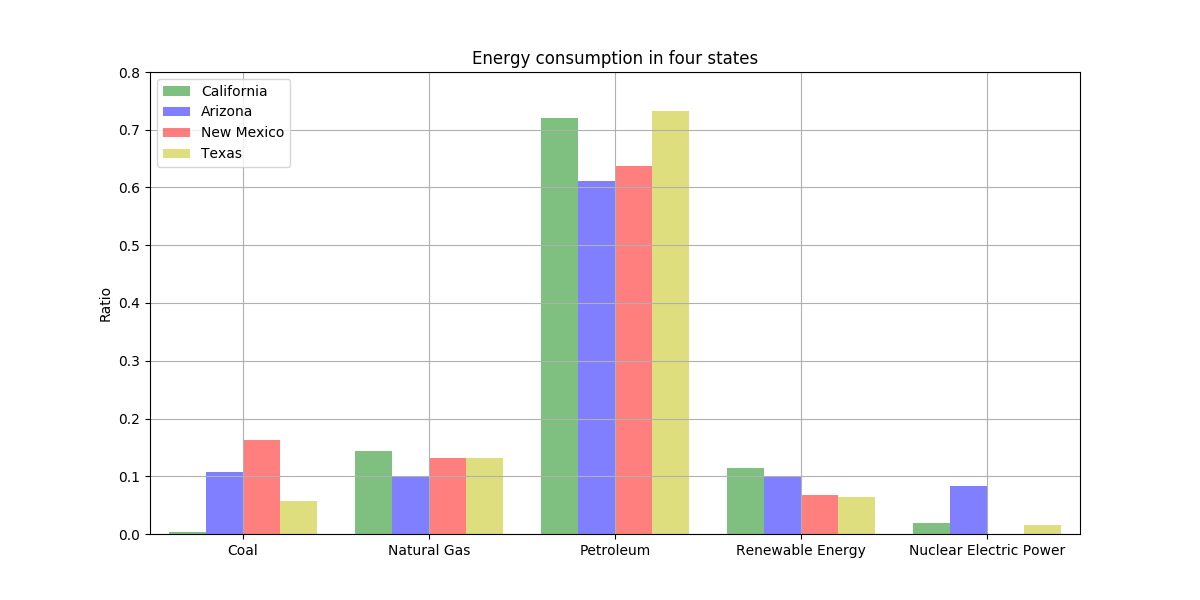
\includegraphics[width=12cm]{energy_2009.png}
\caption{Energy Consumption in 2009} \label{fig:b}
\end{figure}


\begin{table}[!htbp]
\centering
\caption{Evaluate energy profile for four states}\label{tab:aStrangeTable}
\begin{tabular}{ccccc}
\toprule
Standards& California& Arizona& New Mexico& Texas\\
\midrule
CLREVT& 0.27731513& 0.28050433& 0.19956225& 0.21174170 \\
CLREVA& 0.027915380& 0.081253826& 0.077170234& 0.06056389 \\
CLREVC& 0.45310541& 0.40243953& 0.47106859& 0.40201645 \\
CLREVR& 0.44987690& 0.27104287& 0.51764672& 0.26318465 \\
CLREVI& 0.57719885& 0.41052335& 0.54350523& 0.41146144 \\
ECPC& 8.75935762& 15.27066222& 23.891837399& 26.99290274 \\
EI& 447.4832& 589.0200& 885.39466& 1243.675388 \\
\bottomrule
\end{tabular}
\end{table}


\subsection{Evaluate the profiles by criteria }
% 按照标准给每个州打分,然后比较
We rank the four states in these four items and get the state has the best energy profile.
Using this method, the score of California is 22, Arizona's score is 20, New Mexico got 19 and Texas only got 9 points. So the state has best profile of using cleaner, renewable energy is
California.

\section{Predict with Model}
%Based on the historical evolution of energy use in these states, and your understanding of the
% differences between the state profiles you established, predict the energy profile of each state, as
% you have defined it, for 2025 and 2050 in the absence of any policy changes by each governor’s
% office
\subsection{Data collecting and preprocessing}
Based on our model, to predict the energy profile of 2025 and 2050 for each states requires GDP and population of each state.
We found the population prediction of each states, which reference is listed in appendix.
But the GDP prediction doesn't have direct data. So we use the GDP Growth Forecast to calculate the GDP in 2025 and 2050 for each state, assuming their GDP growth is equal to US.
Also assuming the prediction and the calculated data is the value of GDP and population in 2025 and 2050.
\subsection{Predition}
Using the data we collected, the prediction is as follows:
%TODO: Insert the picture.
\begin{table}[!htbp]
\centering
\caption{Forecast 2025}\label{tab:aStrangeTable}
\begin{tabular}{ccccc}
\toprule
Variable& California& Arizona& New Mexico& Texas\\
\midrule
coalVT&	0.0045130156&	0.1763961309&	0.169297041&	0.2130591577 \\
coalVA&	-0.000004245&	-8.06147048353619E-08&	0&	-5.33914224879455E-05\\
coalVC&	0.0008346663&	0.0001074251&	0.0011010455&	0.001901673\\
coalVI&	0.0191793852&	0.0921346145&	0.0073984873&	0.0219831338\\
coalVR&	0.000084605&	1.78386896784993E-05&	0.0002231732&	0.0003992344\\
ngVT&	0.1313055547&	0.0140126102&	0.1194374468&	-0.1391714556\\
ngVA&	0.0041128053&	0.0248502609&	0.1639688911&	-0.0676301499\\
ngVC&	0.1786989652&	0.0666360426&	0.2110454153&	0.0003785705\\
ngVI&	0.2676615396&	0.0109624919&	0.348363306&	-0.2018176788\\
ngVR&	0.3341802182&	0.0476394053&	0.3276451015&	-0.1489412044\\
petroVT&	0.7280296922&	0.5921689547&	0.6597106994&	0.8755059729\\
petroVA&	0.9897102523&	0.9721420506&	0.8304860818&	1.1096712563\\
petroVC&	0.5561812268&	0.6297514699&	0.5461677769&	0.7038169322\\
petroVI&	0.6159945193&	0.6647682217&	0.5560449702&	1.1162868422\\
petroVR&	0.4191970817&	0.6112459226&	0.4457876754&	0.7399625015\\
reVT&	0.1127594008&	0.1056959303&	0.0515542612&	0.0439832704\\
reVA&	0.0061809178&	0.0030060891&	0.0055407405&	-0.0419872122\\
reVC&	0.264284459&	0.3035030454&	0.241677205&	0.2939047459\\
reVI&	0.097164183&	0.2321307086&	0.0881890599&	0.0635477261\\
reVR&	0.246537405&	0.3410948631&	0.2263339065&	0.4085799568\\
nuVT&	0.0233922776&	0.111726182&	0&	0.0066230661 \\
\bottomrule
\end{tabular}
\end{table}

\begin{table}[!htbp]
\centering
\caption{Forecast 2050}\label{tab:aStrangeTable}
\begin{tabular}{ccccc}
\toprule
Variable& California& Arizona& New Mexico& Texas\\
\midrule
coalVT	&	0.0044057668	&	0.1581883234	&	0.1688772331&	0.2130591673	\\
coalVA	&	-3.2295295561E-06	&	-5.3943563074E-08	&	0	&	-5.33914224E-05	\\
coalVC	&	0.000715508	&	9.02716285793421E-05	&	0.0010875846	&	0.001901673	\\
coalVI	&	0.0188992449	&	0.0828377848	&	0.007372724	&	0.0219831338	\\
coalVR	&	7.6279760665E-05	&	1.443782932E-05	&	0.0002197573	&	0.0003992344	\\
ngVT	&	0.1326052795	&	0.0333880189	&	0.1198407186	&	-0.1391714556	\\
ngVA	&	0.0042483122	&	0.030448991	&	0.1630049277	&	-0.0676301499	\\
ngVC	&	0.1779199969	&	0.0817271991	&	0.2115935579	&	0.0003785705	\\
ngVI	&	0.2746156784	&	0.0355198306	&	0.3496955613	&	-0.2018176788	\\
ngVR	&	0.3388485753	&	0.0689002727	&	0.327655832	&	-0.1489412044	\\
petroVT	&	0.7285410102	&	0.6039287042	&	0.6596493911	&	0.8755059729	\\
petroVA	&	0.9880737508	&	0.9638037735	&	0.8314604726	&	1.1096712563	\\
petroVC	&	0.5565722916	&	0.6190745572	&	0.5457112166	&	0.7038169322	\\
petroVI	&	0.6094970796	&	0.665372954	&	0.5548986635	&	1.1162868422	\\
petroVR	&	0.4187213581	&	0.5996497473	&	0.4457327915	&	0.7399625015	\\
reVT	&	0.1118762929	&	0.103826076	&	0.051632124	&	0.0439832704	\\
reVA	&	0.0076808957	&	0.0057454974	&	0.0055303084	&	-0.0419872122	\\
reVC	&	0.2647915166	&	0.2991054419	&	0.2415990793	&	0.2939047459	\\
reVI	&	0.0969876227	&	0.2162654208	&	0.0880288832	&	0.0635477261	\\
reVR	&	0.2423530961	&	0.3314331349	&	0.2263814868	&	0.4085799568	\\
nuVT	&	0.0225715699	&	0.1006686237	&	0	&	0.0066230661	\\
\bottomrule
\end{tabular}
\end{table}

\subsection{Prediction Analysis}
\begin{itemize}
  \item The prediction in 2025
  California's energy agency will not change much and will not rely on coal at all.
  Although oil resources remain his main source of energy, the efficiency of the use of non-renewable resources such as oil will increase as the technology for energy use increases.
  Will not blindly rely on oil resources, such as Tesla cars and so on, so the dependence on oil will be reduced.
  In addition, with the support of current policies, the use of clean and renewable energy sources will further increase, and California is expected to reach its policy goal by 2030.
  Arizona will have a more drastic drop in the use of coal, solar energy and other clean energy will increase the proportion of renewable energy will be larger,
  Arizona's geographical location is very suitable for solar energy and wind energy development and utilization, so for clean energy The use of will be greatly improved.
  The degree of dependence on natural gas and oil and the use of various departments did not change much, did not produce qualitative change, but has already begun to convert clean energy.
  The energy mix in New Mexico is subject to significant changes as the use of clean energy is very small by the year 2009 and the use of clean energy is increasing rapidly and can
  replace some of the natural gas to generate electricity. The demand for coal is further tightened, and the use of oil is still the largest, but because of the increased efficiency of
  the use of petroleum, the total amount of oil used will not increase too fast and the indirect nature will lead to an increase in the proportion of clean energy.
  Texas is one of the four states with the most irrational energy structure. In a short period of time, there is still no way to find the energy of alternative coal,
  so coal will still occupy about $20\%$ of the total consumption. As a result, With a large population and a relatively developed industry,
  consumption in the oil sector continues to rise. In this case, the use of renewable energy and clean energy will continue to shrink.
  Although the total use of clean and renewable energy is on the rise, there is still some way to go to become the most energy-intensive source.
  \item The prediction in 2050
  Energy use in California has entered into a good sustainable development scenario where clean and renewable energy sources have become
  California's major energy sources, but are still being used for oil resources but with increased energy efficiency and promotion of
  clean energy use on the oil only accounts for about $15\%$. Arizona's clean energy can account for almost $60\%$ of total energy,
  the rest mainly oil, the use of oil is still further reduced, the electricity has been provided by all available energy and energy,
  transportation sector can replace the use of oil, then the proportion of oil will drop significantly.
  New Mexico will develop nuclear energy use in the next 30 years, and its share of renewable energy will further increase.
  Together with oil and natural gas, it will become a major part of energy use. Although the coal cannot be completely abandoned,
  the use of coal will decrease Trend, and tend to 0 in the future.
  Texas has made great strides in the use of clean and renewable energy without policy,
  but it is still not a sustainable energy development structure.
  The most important energy sources are still oil and coal the use of descending but also more than $5\%$, clean, renewable energy use accounted for only $35\%$
\end{itemize}


\section{Determine the targets}
% Based on your comparison between the four states, your criteria for “best” profile, and your
% predictions, determine renewable energy usage targets for 2025 and 2050 and state them as goals
% for this new four-state energy compact.
According to the current government work report and the ability of each state to develop their capabilities,
the goals of the four states are set first, and then the tasks are allocated according to the capabilities of each state.
In the pre-development phase of the exchange of science and technology and the use of funds, It's better than before, especially for Texas.
\begin{itemize}
  \item 2025 Targets: Decrease use of coal by $20\%$, increase energy intensity by $34\%$, and raise the use of clean energy by $37\%$.
  \item Target 2050: Completely unsuitable for coal, doubling energy intensity compared to 2009,
  achieving over $50\%$ clean energy and becoming a major source of energy in a state.
\end{itemize}
\section{Propose measures}
% Identify and discuss at least three actions the four states might take to meet their energy
% compact goals.
\begin{itemize}
  \item Reduce electricity and natural gas consumption by improving energy efficiency and reducing demand
        Targets can be reached through a variety of measures, including enhanced appliance standards,
        efficiency improvements in public buildings, and financial incentives for retail customers.
  \item The government should formulate policies to support renewable energy to prioritize and subsidize grid systems
  Such policies, now in place in about 50 countries, include priority dispatch for electricity from renewable sources and special feed-in tariffs, quota obligations and energy tax exemptions.
  Most of the electricity demand is the continuous and reliable power supply, traditionally provided by basic load power generation. Some of them are based on a wide range of predictable requirements for shorter periods (such as peak loads).
  Therefore, if renewable energy is connected to the grid, there will be a problem of reserve capacity.
  \item Vigorously develop solar power generation technology to reduce transmission losses
The obvious advantage of solar and, to some extent, other renewable energy systems is that they are distributed and may be close to demand, so transmission losses can be reduced if traditional power plants are far apart.
These four states can improve technology, such as the use of photovoltaic (PV) systems and the use of concentrating solar photovoltaic (CPV) for greater efficiency.
  \item Reduce the intermittent problems of water system power generation, improve energy efficiency
  The main advantage of hydraulic systems is their ability to handle seasonal (and daily) peak loads. In practice, the use of stored water is sometimes complicated by irrigation needs, which may not be in sync with the peak of electricity demand.
One way to reduce intermittency is to produce hydrogen by electrolysis and send it to the gas grid.
  \item Development and use of nuclear energy and hydrogen energy
  Nuclear energy is a low-carbon energy and has a very small environmental impact.
Hydrogen is widely recognized as a possible transport fuel if certain problems can be economically overcome.
It can be used in conventional combustion engines as well as in fuel cells to convert chemical energy directly into electrical energy without normal combustion.
For intermittent renewable energy sources, such as solar and wind energy,
matching production to grid requirements is very difficult and it is obviously not possible to exceed $20\%$ of the total electricity supply.
However, if these sources are used to make hydrogen, they can be fully utilized whenever there is a chance.
In a broad sense, it does not matter if it is cut in or cut out, and hydrogen is stored and used only as needed.
\end{itemize}

% 摘要
\begin{thebibliography} {99}
  % \bibitem{1} D.~E. KNUTH   The \TeX{}book  the American
  % Mathematical Society and Addison-Wesley
  % Publishing Company , 1984-1986.
  \bibitem{1}\url{https://www.eia.gov/state/seds/seds-technical-notes-complete.php?sid=US#Consumption}
  \bibitem{2} Joel Darmstadter  Energy and Population September 2004 Issue Brief 04–01
  \bibitem{3}\url{http://reliawiki.org/index.php/Multiple_Linear_Regression_Analysis}
  \bibitem{4}\url{https://en.wikipedia.org/wiki/Normalization_(statistics)}
  \bibitem{5}\url{https://en.wikipedia.org/wiki/Energy_intensity}
\end{thebibliography}

\end{document}
